\chapter{Grupo III}
\section{Objectivo}
O objectivo principal deste grupo era usar o modo de cifras por blocos ECB em imagens, mais propriamente em imagens que são guardadas como uma matriz de pontos não comprimidas (\textit{bitmap images}). No final, pretendia-se verificar que neste modo é possível retirar informação útil do criptograma, ou seja, é possível verificar certos padrões da imagem original no criptograma.
%
\section{Bitmap image}
Existem vários formatos de \textit{bitmap images}, tais como \textsf{GIF}, \textsf{PNG}, \textsf{TIFF} ou \textsf{JPEG}. Mas nenhum destes formatos serve para o propósito deste grupo, pois são formatos comprimidos. Um outro formato mais conhecido em ambientes \textit{Windows} é o \textsf{BMP}.
Existem várias formas de representar um \verb|BMP|, sendo que é comum a todas elas é o facto de no início do ficheiro estar o cabeçalho. De seguida apresenta-se o formato de um cabeçalho:
\begin{center}
\begin{tabular}{| c | c | p{7cm} |}
  \hline
  \textbf{Posição} & \textbf{Tamanho} & \textbf{Descrição} \\
  \hline
  0x0 & 2 bytes & Serve para identificar o tipo de imagem (normalmente é 0x42 que equivale a \textsf{BMP}) \\
  \hline
  0x2 & 4 bytes & Tamanho do ficheiro em bytes \\
  \hline
  0x6 & 2 bytes & Reservado; depende da aplicação que cria a imagem \\
  \hline
  0x8 & 2 bytes & Reservado; depende da aplicação que cria a imagem \\
  \hline
  0xA & 4 bytes & Indica em que posição começa a matriz de pontos \\
  \hline
\end{tabular}
\end{center}
No âmbito deste trabalho, a informação que mais nos interessa é a posição em que começa a matriz de pontos. Sendo assim, os passos a seguir são:
\begin{enumerate}
  \item Abrir a imagem em modo hexadecimal
  \item Obter a posição onde se encontra a matriz de pontos
  \item Cifrar imagem original em modo ECB
  \item Tendo a imagem cifrada, copiar o conteúdo do cabeçalho da imagem original para o criptograma, caso contrário a imagem não é reconhecida por nenhum leitor de imagens
\end{enumerate}
%
\section{Implementação}
Para se obter o resultado das operações descritas anteriormente, são fundamentalmente precisas três ferramentas:
\begin{description}
  \item[od] Para abrir um ficheiro em modo hexadecimal, podendo assim manipulá-lo \textit{byte} a \textit{byte}
  \item[OpenSSL] Para cifrar a imagem em modo ECB
  \item[dd] Para copiar certas quantidades de \textit{bytes} de um ficheiro para outro
\end{description}
Estas três ferramentas são combinadas entre si usando vários comandos \textsf{Bash} tais como \verb|head|, \verb|tail| ou o redireccionamento de \textit{streams}.\\
Para se obter a posição inicial da matriz de pontos, usa-se o seguinte comando:
\begin{lstlisting}[style=Bash]
od -t x -An $IFILE  | head -n1 | cut -d' ' -f4,5 | tr -d ' ' | tail -c15 | cut -c1-8
\end{lstlisting}
De seguida explica-se o que cada um dos comandos faz:
\begin{description}
  \item[od -t x -An] lê todo o ficheiro \verb|$IFILE| em modo hexadecimal
  \item[head -n1] apresenta apenas a primeira linha do ficheiro; essa primeira linha contém os primeiros 16 \textit{bytes} do ficheiro, representados por 4 blocos de 4 \textit{bytes}. Vamos usar os seguintes 16 \textit{bytes} como exemplo a partir de agora: \verb|687a4d42 00000010 007a0000 006c0000|
  \item[cut -d' ' -f4,5] para se obterem os terceiro e quarto blocos de \textit{bytes}. No exemplo, obtém-se \verb|007a0000 006c0000|
  \item[tr -d ' '] apagar os espaços em branco. Fica-se com \verb|007a0000006c0000|
  \item[tail -c15] obtem os últimos 15 caractéres (ou seja, 7 \textit{bytes} e um \verb|\n|). Fica-se com \verb|7a0000006c0000|
  \item[cut -c1-8] obtem os primeiros 8 caractéres, ou seja, 4 \textit{bytes}. Fica-se com \verb|7a000000|
\end{description}
O resultado obtido anteriormente está no formato \textit{little endian}, ou seja, é necessário convertê-lo para \textit{big endian}, para depois o converter para decimal. Eis como o fizemos no nosso script, estando em \verb|$HEADERSIZE_LE| o resultado anterior \verb|7a000000|:
\begin{lstlisting}[style=Bash]
HEADERSIZE=""
for (( i = 0; i < ${#HEADERSIZE_LE}; i+=2 )); do
  BYTE=${HEADERSIZE_LE:$i:2} # get substring starting in $i with 2 chars
  HEADERSIZE=$BYTE$HEADERSIZE
done
# convert header size to decimal
HEADERSIZE=$(echo "obase=10; ibase=16; $HEADERSIZE" | bc)
\end{lstlisting}
No exemplo anterior, o valor de \verb|HEADERSIZE| é 122.\\
Nesta altura, já podemos cifrar a matriz de pontos. Para isso usamos o \textsf{dd} para obter e cifrar apenas os \textit{bytes} necessários.\\
Em primeiro lugar, copiámos apenas o \textit{header} da imagem original para o ficheiro de destino \verb|OFILE|.
\begin{lstlisting}[style=bash]
dd if="$IFILE" of="$OFILE" bs=1 count="$HEADERSIZE" conv=notrunc 2> /dev/null
\end{lstlisting}
De seguida, ciframos a matriz de pontos e redireccionámos o resultado para o ficheiro de destino. A matriz de pontos de pontos é lida directamente a partir do ficheiro original, usando também o \textsf{dd}, e o seu resultado é enviado através do \textsf{stdin} para o \textsf{OpenSSL}.
\begin{lstlisting}[style=bash]
dd if="$IFILE" bs=1 skip="$HEADERSIZE" conv=notrunc 2> /dev/null | openssl enc -e "$CIPHER" >> "$OFILE"
\end{lstlisting}
De forma a automatizar este processo, criou-se um pequeno \textit{script} em \textsf{Bash}. O Código~\ref{ecb:script} e a sua invocação é a seguinte:
\begin{lstlisting}[style=Bash]
$ ./script infile.bmp outfile.bmp ecb-cipher
$ ./script car.bmp car-des.bmp -des-ecb
\end{lstlisting}
\begin{lstlisting}[style=Bash,caption={\textit{Script} utilizado para cifrar imagens com uma cifra por blocos.},label=ecb:script]
#!/bin/bash

usage() {
  echo "Chamaste mal o script"
  exit
}

if [ -z "$1" ] || [ -z "$2" ] || [ -z "$3" ]; then
  usage
fi
IFILE="$1"
if [ ! -f "$IFILE" ]; then
  echo $IFILE" does not exist."
  exit
fi
OFILE="$2"
if [ -f "$OFILE" ]; then
  echo $OFILE" already exists. Cannot proceed"
  exit
fi
CIPHER="$3"

HEADERSIZE_LE=$(od -t x -An "$IFILE" | head -n1 | \
  cut -d' ' -f4,5 | tr -d ' ' | tail -c15 | cut -c1-8)
HEADERSIZE_LE="${HEADERSIZE_LE^^}"

HEADERSIZE=""
for (( i = 0; i < ${#HEADERSIZE_LE}; i+=2 )); do
  BYTE=${HEADERSIZE_LE:$i:2}
  HEADERSIZE=$BYTE$HEADERSIZE
done
HEADERSIZE=$(echo "obase=10; ibase=16; $HEADERSIZE" | bc)
echo "Header size of '"$IFILE"' is "$HEADERSIZE" bytes, located at position 0x0A"

dd if="$IFILE" of="$OFILE" bs=1 count="$HEADERSIZE" \
  conv=notrunc 2> /dev/null

dd if="$IFILE" bs=1 skip="$HEADERSIZE" \
  conv=notrunc 2> /dev/null | \
  openssl enc -e "$CIPHER" >> "$OFILE"
\end{lstlisting}
\section{Exemplos e conclusões}
Decidimos usar como exemplos as seguintes imagens:
\begin{figure}[htb]
\centering
\subfigure[Famosa imagem do pinguim]{
\includegraphics[scale=0.45, keepaspectratio = true]{img/penguin}}
\subfigure[Carro]{
\includegraphics[scale=0.35, keepaspectratio = true]{img/car}}
\caption{Exemplos utilizados}
\end{figure}
Vamos cifrar com DES e com AES para ver se existem diferenças claras entre ambas. Em todas elas, a \textit{passphrase} utilizada é \textsf{passphrase-quase-quase-boa-para-usar-com-o-modo-ecb}.\\
Cifrando com o DES e AES, obtêm-se os seguintes resultados:
\begin{figure}[htb]
\centering
\subfigure[Pinguim, utilizando o comando \texttt{./script penguin.bmp penguin-des.bmp -des-ecb}]{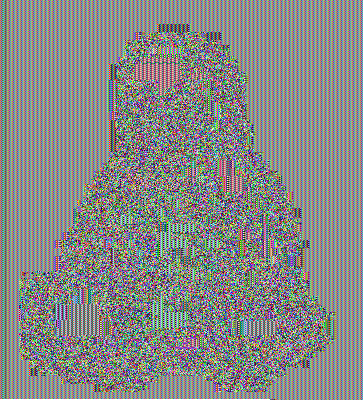
\includegraphics[scale=0.45, keepaspectratio = true]{img/penguin-des}}
\subfigure[Carro, utilizando o comando \texttt{./script car.bmp car-des.bmp -des-ecb}]{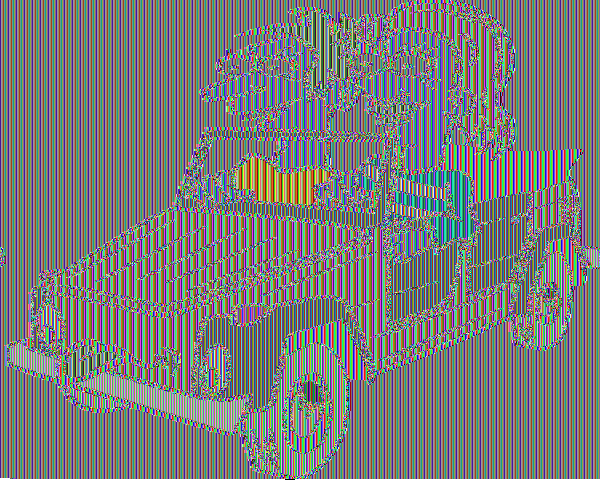
\includegraphics[scale=0.35, keepaspectratio = true]{img/car-des}}
\caption{Cifração com DES em modo ECB}
\end{figure}
%
\begin{figure}[htb]
\centering
\subfigure[Pinguim, utilizando o comando \texttt{./script penguin.bmp penguin-aes192.bmp -aes-192-ecb}]{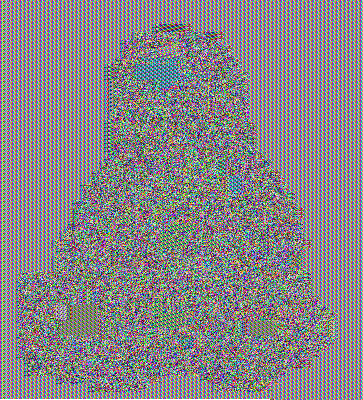
\includegraphics[scale=0.45, keepaspectratio = true]{img/penguin-aes192}}
\subfigure[Pinguim, utilizando o comando \texttt{./script penguin.bmp penguin-aes192.bmp -aes-192-ecb}]{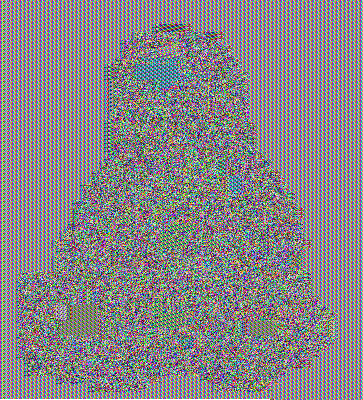
\includegraphics[scale=0.45, keepaspectratio = true]{img/penguin-aes192}}
\subfigure[Carro, utilizando o comando \texttt{./script car.bmp car-aes192.bmp -aes-256-ecb}]{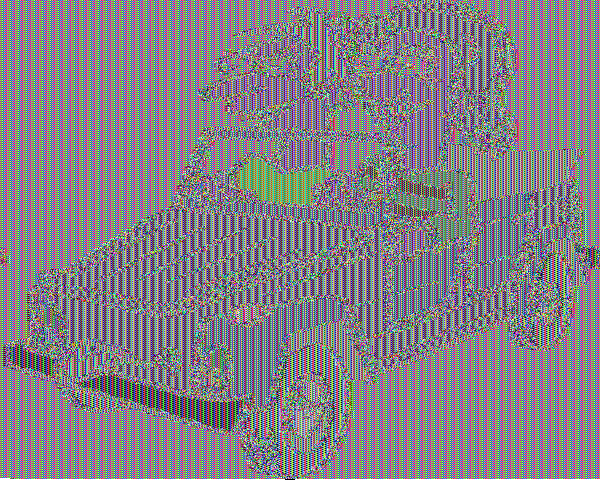
\includegraphics[scale=0.35, keepaspectratio = true]{img/car-aes256}}
\subfigure[Carro, utilizando o comando \texttt{./script car.bmp car-aes192.bmp -aes-256-ecb}]{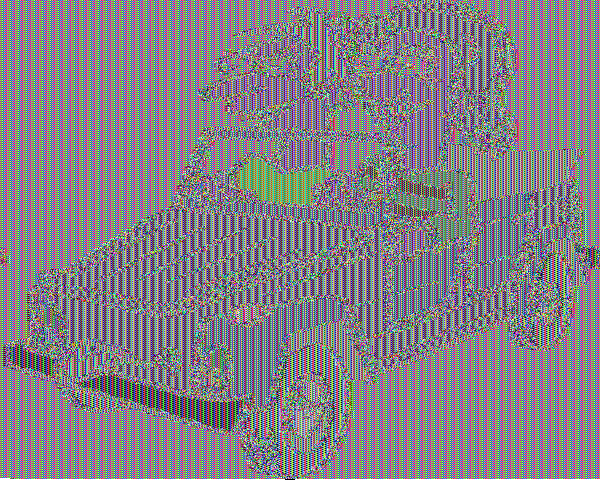
\includegraphics[scale=0.35, keepaspectratio = true]{img/car-aes256}}
\caption{Cifração com AES em modo ECB, com 192 e 256 bits}
\end{figure}
%
Como se pode ver, não existe uma diferença clara entre o AES e o DES. Da mesma forma, também não existe nenhuma diferença entre o AES com 192 e 256 bits. No entanto, é claro que em todas as cifras, em conjunto com o ECB, é possível encontrar certos padrões da mensagem original.
%
%\begin{btSect}{bib/bibz03}
% \section{Bibliografia}
 %\btPrintCited
 %\btPrintNotCited
% \btPrintAll
%\end{btSect}